% ============================================================================
% DevBridge -- Module 6: The Skill Graph
% Technical report on the skill-graph layer (submodules 6.0-6.5).
%
% Compile with pdflatex (two passes for the table of contents / references):
%   pdflatex module6-skill-graph-report.tex
%   pdflatex module6-skill-graph-report.tex
%
% Uses only packages that ship with any standard TeX Live / MiKTeX
% installation (psnfss, tools, graphics, tikz, hyperref). No fontspec, no
% XeLaTeX/LuaLaTeX required -- this compiles under plain pdflatex.
% ============================================================================
\documentclass[11pt,a4paper]{article}

% ---- fonts & encoding -------------------------------------------------------
\usepackage[T1]{fontenc}
\usepackage[utf8]{inputenc}
\usepackage{mathpazo}                 % Palatino text + math
\usepackage[scaled=0.92]{helvet}      % Helvetica for sans (headings)
\usepackage{microtype}

% ---- layout ------------------------------------------------------------------
\usepackage[a4paper,margin=2.4cm,headheight=14pt]{geometry}
\usepackage{fancyhdr}
\usepackage{titlesec}
\usepackage{enumitem}
\setlist[itemize]{leftmargin=1.3em, itemsep=2pt, topsep=3pt}
\setlist[enumerate]{leftmargin=1.5em, itemsep=2pt, topsep=3pt}

% ---- math, tables, color, graphics --------------------------------------------
\usepackage{amsmath,amssymb}
\usepackage{array}
\usepackage{booktabs}
\usepackage{longtable}
\usepackage{float}
\usepackage{xcolor}
\usepackage{graphicx}
\usepackage{tikz}
\usetikzlibrary{arrows.meta,positioning,calc,decorations.pathreplacing}
\usepackage{framed}   % colored/ruled boxes that may contain arbitrary
                       % multi-paragraph content (align*, lists, ...) --
                       % unlike \colorbox or a tikz \node{...}, framed's
                       % \MakeFramed/\endMakeFramed do not grab their body as
                       % a single delimited argument, so splitting them across
                       % a \newenvironment's before/after text is safe.

% ---- hyperref (load late) -----------------------------------------------------
\usepackage[colorlinks=true,linkcolor=accentlink,citecolor=accentlink,
            urlcolor=accentlink,pdfborder={0 0 0}]{hyperref}

% ============================================================================
% Palette -- carried over from the module's own artifact write-up.
% ============================================================================
\definecolor{accent}{HTML}{1C6A5E}     % pine teal -- the module's accent
\definecolor{accent2}{HTML}{2E8C7C}
\definecolor{accentlink}{HTML}{15544A}
\definecolor{negative}{HTML}{9C4A21}   % rust -- reserved for negative evidence
\definecolor{warn}{HTML}{8A6A17}
\definecolor{inkgray}{HTML}{3E4A46}
\definecolor{mutedgray}{HTML}{6B7772}
\definecolor{rulegray}{HTML}{C2CEC8}
\definecolor{bandfill}{HTML}{DCEAE6}
\definecolor{sunken}{HTML}{EBF0ED}
\colorlet{shadecolor}{sunken}   % background used by framed's \shaded environment

% ============================================================================
% Math operators
% ============================================================================
\DeclareMathOperator{\logit}{logit}
\DeclareMathOperator{\sig}{sigmoid}

% ============================================================================
% Section styling (sans, accent-colored, ruled)
% ============================================================================
\titleformat{\section}
  {\normalfont\sffamily\Large\bfseries\color{accent}}
  {\thesection}{0.6em}{}[{\color{rulegray}\titlerule[1pt]}]
\titleformat{\subsection}
  {\normalfont\sffamily\large\bfseries\color{inkgray}}
  {\thesubsection}{0.5em}{}
\titleformat{\subsubsection}
  {\normalfont\sffamily\bfseries\color{inkgray}}
  {\thesubsubsection}{0.5em}{}
\titlespacing*{\section}{0pt}{1.6em}{0.9em}
\titlespacing*{\subsection}{0pt}{1.3em}{0.5em}
\titlespacing*{\subsubsection}{0pt}{1.0em}{0.3em}

\pagestyle{fancy}
\fancyhf{}
\renewcommand{\headrulewidth}{0.4pt}
\renewcommand{\footrulewidth}{0pt}
\fancyhead[L]{\small\sffamily\color{mutedgray}DevBridge -- Module 6}
\fancyhead[R]{\small\sffamily\color{mutedgray}The Skill Graph}
\fancyfoot[C]{\small\sffamily\color{mutedgray}\thepage}

% ============================================================================
% Small helper macros
% ============================================================================

% A colored tag, e.g. [S4] next to a subsection title about the model.
\newcommand{\modeltag}[1]{%
  {\sffamily\footnotesize\bfseries\color{accent}%
   \fboxsep=2pt\fbox{\color{accent}#1}}%
}

% A boxed key equation -- used sparingly, for the handful of headline formulas.
% framed's `shaded` environment (background tinted by \colorlet{shadecolor}{sunken}
% above) is built for exactly this: a colored background behind arbitrary
% multi-line content, including align*/alignat*. It does not grab its body as
% a delimited argument, unlike \colorbox or a tikz node, so it is safe to use
% directly inside a \newenvironment whose real content sits between \begin/\end.
\newenvironment{keyeq}{%
  \begin{shaded}
  \centering
}{%
  \end{shaded}
}

% A callout box for limitations / notices, with a colored left rule -- built
% directly on framed's own \MakeFramed/\FrameCommand primitives (the same
% mechanism behind its ready-made `leftbar` environment), so the rule color
% can be set without the argument-grabbing hazard described above.
\newenvironment{notebox}[1]{%
  \def\FrameCommand{{\color{warn}\vrule width 2.4pt}\hspace{9pt}}%
  \MakeFramed{\advance\hsize-\width \FrameRestore}%
  \noindent{\sffamily\footnotesize\bfseries\color{warn}#1}\par\smallskip
  \small
}{%
  \par\endMakeFramed
}

% A refusal / open-item row list -- label + description.
\newcommand{\pointitem}[2]{%
  \par\noindent{\sffamily\bfseries\color{inkgray}#1}\par
  \noindent{\small #2}\par\addvspace{0.55em}
}

\newcolumntype{L}[1]{>{\raggedright\arraybackslash}p{#1}}
\newcolumntype{R}[1]{>{\raggedleft\arraybackslash}p{#1}}
\newcolumntype{C}[1]{>{\centering\arraybackslash}p{#1}}

% ============================================================================
\begin{document}

% ---------------------------------------------------------------------------
\begin{titlepage}
\centering
\vspace*{2.2cm}
{\sffamily\footnotesize\bfseries\color{mutedgray}\MakeUppercase{DevBridge --
Verified-Talent Freelance Platform}}\\[1.6cm]

{\sffamily\Huge\bfseries\color{accent} The Skill Graph}\\[0.5cm]
{\sffamily\Large\color{inkgray} Module 6: Technical Report}\\[2.2cm]

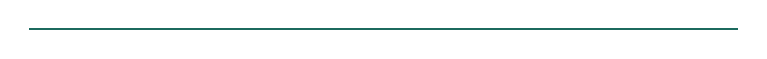
\begin{tikzpicture}
\draw[accent, line width=1pt] (0,0) -- (9,0);
\end{tikzpicture}
\vspace{1.4cm}

{\sffamily\normalsize\color{inkgray}
Module 6 takes a verification report about one developer and produces a
per-skill \emph{belief}: not a rating, but a Gaussian over ability that widens
when evidence is thin and widens again as evidence ages. This report names
every model in the layer, states every free constant, and walks the scoring
model through one real number, start to finish.}

\vspace{2.6cm}

\begin{tabular}{ll}
\sffamily\bfseries\color{mutedgray} Author        & \emph{[Module 6 owner --- fill in name / roll number]} \\[4pt]
\sffamily\bfseries\color{mutedgray} Module         & M6 --- Skill Graph (of six planned platform modules) \\[4pt]
\sffamily\bfseries\color{mutedgray} Contracts      & \texttt{m6-parameters.yaml} v1.0.0, \texttt{ontology-seed.yaml} v0.1.0 \\[4pt]
\sffamily\bfseries\color{mutedgray} Test status    & 562 tests passing, 0 failing \\[4pt]
\sffamily\bfseries\color{mutedgray} Date           & \today \\
\end{tabular}

\vfill
{\small\color{mutedgray}\sffamily Every figure in this report is reproduced
from the committed source of Module 6, not quoted from a design document.}
\end{titlepage}

\tableofcontents
\thispagestyle{empty}
\newpage

% ============================================================================
\section{Before Anything Else: Three Refusals}
% ============================================================================

Module 6 is easiest to understand by what it declines to do. Each refusal
below is enforced by code and held by a test suite, not written down and
hoped for; the design of every later section follows from these three.

\pointitem{Nothing here is trained.}{No model is fitted, no optimiser runs,
no labelled data exists anywhere in the module. Every constant is declared in
a contract file (\texttt{contracts/m6-parameters.yaml}) with a stated reason
and a sensitivity-sweep range. The update rule is closed-form Kalman
arithmetic --- arithmetic a reviewer can check by hand, which is the point.}

\pointitem{There is no overall score.}{Ability is per-skill or it is
nothing. The endpoint \texttt{GET /developers/\{ref\}/score} returns
\texttt{400} with an explanation, permanently. A single aggregate number
would collapse an interval-valued, per-skill, decaying belief into something
that reads like a credit rating.}

\pointitem{The language model never judges.}{Upstream, in Module 5, a large
language model normalises free-text CV content into structured claims. It
never assigns a score, a weight, or a verdict. Everything downstream of a
claim is deterministic arithmetic over declared constants.}

% ============================================================================
\section{Architecture: Six Submodules, One Direction}
% ============================================================================

Evidence flows one way through the layer. The ontology (6.1) is consulted by
three stages but never receives anything back from them. Integrity analytics
(6.5) reads the evidence log and the scored states, and writes nothing at
all -- which is what lets it stay entirely outside the scoring path.

\begin{table}[H]
\centering\small
\begin{tabular}{@{}llL{8.6cm}@{}}
\toprule
\textbf{Submodule} & \textbf{Package} & \textbf{Responsibility} \\
\midrule
6.0 & \texttt{m6\_projection} & Verified artefacts $\to$ evidence events (the rule table, Section~\ref{sec:projection}) \\
6.1 & \texttt{m6\_ontology}   & Skills, volatility tiers, typed relations (Section~\ref{sec:ontology}) \\
6.2 & \texttt{m6\_ingestor}   & Validation, consent, idempotency, append-only log (Section~\ref{sec:ingestor}) \\
6.3 & \texttt{m6\_scoring}    & The Bayesian filter: observation, update, decay, propagation (Section~\ref{sec:scoring}) \\
6.4 & \texttt{m6\_query}      & Intervals, the \texttt{explain} endpoint, tiered search (Section~\ref{sec:query}) \\
6.5 & \texttt{m6\_integrity}  & Findings about the shape of the evidence; changes no score (Section~\ref{sec:integrity}) \\
\bottomrule
\end{tabular}
\caption{The six submodules of Module 6 and the package each lives in.}
\end{table}

\begin{figure}[H]
\centering
% The picture's own coordinates run out to x=16.2 with node widths on top of
% that, so it is very slightly wider than \textwidth at 1:1 scale -- resizebox
% guarantees it fits regardless of exact node-label metrics.
\resizebox{\textwidth}{!}{%
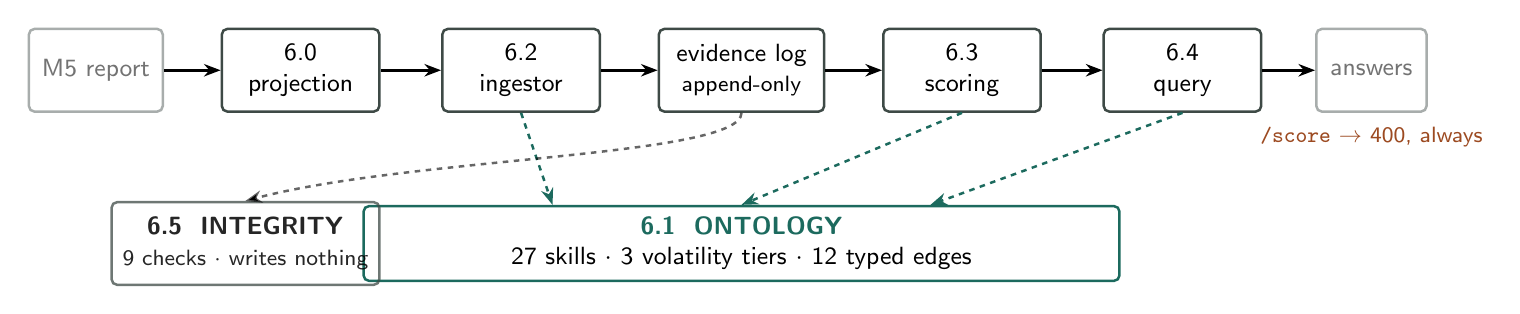
\begin{tikzpicture}[
    box/.style={draw=inkgray, line width=0.9pt, rounded corners=2pt,
                minimum height=1.05cm, align=center, font=\sffamily\small},
    faint/.style={draw=inkgray, line width=0.9pt, rounded corners=2pt,
                  minimum height=1.05cm, align=center, font=\sffamily\small,
                  draw opacity=0.45, text opacity=0.55},
    onto/.style={draw=accent, line width=0.9pt, rounded corners=2pt,
                 minimum height=0.95cm, align=center, font=\sffamily\small},
    arr/.style={-{Stealth[length=6pt]}, line width=0.9pt},
    ontoarr/.style={-{Stealth[length=6pt]}, line width=0.9pt, accent,
                    dash pattern=on 2pt off 2pt},
  ]
  \node[faint, minimum width=1.7cm]           (m5)  at (0,0)    {M5 report};
  \node[box, minimum width=2.0cm]             (p)   at (2.6,0)  {6.0\\ projection};
  \node[box, minimum width=2.0cm]             (ing) at (5.4,0)  {6.2\\ ingestor};
  \node[box, minimum width=2.1cm]             (log) at (8.2,0)  {evidence log\\ \footnotesize append-only};
  \node[box, minimum width=2.0cm]             (sc)  at (11.0,0) {6.3\\ scoring};
  \node[box, minimum width=2.0cm]             (q)   at (13.8,0) {6.4\\ query};
  \node[faint, minimum width=1.4cm]           (ans) at (16.2,0) {answers};

  \draw[arr] (m5) -- (p);
  \draw[arr] (p)  -- (ing);
  \draw[arr] (ing)-- (log);
  \draw[arr] (log)-- (sc);
  \draw[arr] (sc) -- (q);
  \draw[arr] (q)  -- (ans);

  \node[onto, minimum width=9.6cm] (onto) at (8.2,-2.2)
       {\textbf{\color{accent}6.1 \ ONTOLOGY} \\ 27 skills $\cdot$ 3 volatility tiers $\cdot$ 12 typed edges};
  \draw[ontoarr] (ing.south) -- ([xshift=-2.4cm]onto.north);
  \draw[ontoarr] (sc.south)  -- (onto.north);
  \draw[ontoarr] (q.south)   -- ([xshift=2.4cm]onto.north);

  \node[box, draw opacity=0.75, text opacity=0.85, minimum width=3.4cm]
       (integ) at (1.9,-2.2) {\textbf{6.5 \ INTEGRITY} \\ \footnotesize 9 checks $\cdot$ writes nothing};
  \draw[arr, dash pattern=on 2pt off 2pt, draw opacity=0.6]
       (log.south) .. controls (8.2,-1.1) and (4.0,-1.1) .. (integ.north);

  \node[negative, font=\sffamily\footnotesize] at (16.2,-0.85)
       {\texttt{/score} $\to$ 400, always};
\end{tikzpicture}%
}
\caption{The one-way pipeline. The dashed teal arrows are the only thing 6.1
exposes: three read-only questions. 6.2 may ask \texttt{knows()} and nothing
else -- if the ingestor could reach the relation edges, propagation would
migrate from read time (6.3, where it can be switched off and explained) to
write time, where it cannot.}
\label{fig:pipeline}
\end{figure}

% ============================================================================
\section{Model 1: The Event Projection Rule Table (6.0)}
\label{sec:projection}
% ============================================================================

The first model in the layer is not statistical, and saying so plainly
matters. It is a \textbf{declared lookup table} mapping each kind of
verified artefact to three numbers: how strong a signal it is, how much the
source can be trusted, and which skills it bears on. Nothing here is
inferred; the table lives in \texttt{contracts/projection-rules.yaml} and a
reviewer can disagree with any single row of it.

\begin{table}[H]
\centering\small
\begin{tabular}{@{}lL{5.1cm}ccl@{}}
\toprule
\textbf{Evidence kind} & \textbf{Emitted when} & \textbf{strength} & \textbf{reliability} & \textbf{direction} \\
\midrule
\texttt{platform\_rating}     & handle resolves and a max rating exists                    & 0.80 & 0.90 & positive \\
\texttt{repo\_artifact}       & repo exists, owner matches, not a fork or shell             & $0.45{+}0.05{\cdot}\text{band}$ & 0.70 & positive \\
\texttt{claim\_corroborated}  & a CV skill claim is matched by verified evidence            & 0.70 & 0.80 & positive \\
\texttt{artifact\_live}       & a deployment responds                                       & 0.40 & 0.85 & positive \\
\texttt{credential\_verified} & the issuer confirms the credential                          & 0.60 & 0.95 & positive \\
\texttt{cv\_claim}            & a claim with no corroboration anywhere                      & 0.30 & 0.20 & positive \\
\texttt{claim\_contradicted}  & a decisive check fails against a skill claim                & 0.90 & 0.95 & {\color{negative}negative} \\
\bottomrule
\end{tabular}
\caption{The seven emit rules. \texttt{strength} and \texttt{reliability}
travel on the event and enter the scoring model's variance term
(Section~\ref{sec:s3}); nothing else about the artefact does.}
\end{table}

\subsection*{Reliability factors, named on the event}

Reliability is multiplied by discount factors, each recorded on the event by
name, so a candidate who asks why a number is low gets the factor, not a
total.

\begin{keyeq}
\[
\text{reliability} = \text{reliability\_base} \times \!\!\prod \text{factors}
\]
\end{keyeq}

\begin{table}[H]
\centering\small
\begin{tabular}{@{}lcL{8.3cm}@{}}
\toprule
\textbf{Factor} & \textbf{Value} & \textbf{Applies to} \\
\midrule
\texttt{ownership\_unverified}      & $\times\,0.6$ & the GitHub identity is self-claimed, not proven (positive-direction events only) \\
\texttt{scraped\_source}            & $\times\,0.7$ & a profile page was parsed, not an API queried \\
\texttt{aggregate\_across\_sources} & $\times\,0.7$ & the claim pools a count no single source can confirm \\
\texttt{stale\_evidence}            & $\times\,1.0$ & deliberately inert --- decay handles age at scoring time \\
\bottomrule
\end{tabular}
\caption{Reliability discount factors from
\texttt{contracts/projection-rules.yaml}.}
\end{table}

\texttt{ownership\_unverified} applies only to evidence that would
\emph{raise} a score. A self-claimed account that contradicts the CV is
credible --- nobody volunteers a handle that undermines them --- so the
discount is asymmetric on purpose. \texttt{stale\_evidence} exists and does
nothing: applying an age discount here as well as in the decay kernel
(Section~\ref{sec:s5}) would count staleness twice, and the contract records
the zero explicitly so nobody re-enables it later.

\begin{notebox}{A rule with teeth}
Every claim must end up either carried by an event or named in
\texttt{not\_emitted[]} with a reason. Silence is not an available outcome.
This invariant is checked at projection time, and when it was added it
immediately caught two claim kinds that had been vanishing without trace: a
\texttt{certification} claim, and an uncorroborated \texttt{project} claim.
\end{notebox}

% ============================================================================
\section{Models 2 and 3: The Skill Graph (6.1) and the Absence of a Model (6.2)}
\label{sec:ontology}
\label{sec:ingestor}
% ============================================================================

\subsection*{Model 2 --- The Volatility-Tier Model}

Every skill is filed in one of three tiers, and the tier --- not the
candidate, not the evidence --- fixes how fast a signal about it goes stale.
Three tiers rather than a continuum, because a continuum is a parameter per
skill and cannot be defended or swept.

\begin{table}[H]
\centering\small
\begin{tabular}{@{}lcccL{4.4cm}@{}}
\toprule
\textbf{Tier} & $\lambda$ per day & $\tau=k/\lambda$ & true half-life $\tau\ln 2$ & Example skills \\
\midrule
fundamental & $1.0\times10^{-4}$ & 3500 d & 2426 d & algorithms, C++, data structures \\
ecosystem   & $3.0\times10^{-4}$ & 1167 d & 809 d  & Python, TypeScript, Go, SQL \\
framework   & $7.5\times10^{-4}$ & 467 d  & 324 d  & React, Docker, PostgreSQL \\
\bottomrule
\end{tabular}
\caption{The three volatility tiers, from \texttt{contracts/m6-parameters.yaml}.}
\end{table}

Someone who could reason about algorithms in 2019 still can; a framework
signal from three years ago genuinely means less. Getting a tier wrong is
the difference between a skill that fades in a year and one that holds for a
decade, so tiers are reviewed in a YAML file rather than set in code.

\begin{notebox}{Naming discrepancy, flagged not hidden}
The contract calls $k/\lambda$ the half-life, and the API publishes it as
\texttt{half\_life\_days}. Strictly it is the \emph{e-folding time constant}
$\tau$: at $t=\tau$ the mean has moved $63.2\%$ of the way back to the
prior, not $50\%$. The true half-life is $\tau\ln 2$ --- the fourth column
above. The arithmetic is correct everywhere; only the label is loose, and
the fix is a rename rather than a change of behaviour.
\end{notebox}

\subsection*{Model 3 --- The Relation Model}

Twelve directed, typed edges. An edge asserts that evidence for one skill is
genuine evidence about another --- a strong thing to claim, so the graph is
deliberately sparse and every hop is damped. The type carries the damping
coefficient $\gamma$; there is one $\gamma$ per \emph{type}, never per edge,
because per-edge coefficients are an unbounded parameter space nobody could
sweep or defend.

\begin{table}[H]
\centering\small
\begin{tabular}{@{}lcL{7.2cm}@{}}
\toprule
\textbf{Edge type} & $\gamma$ & \textbf{Example} \\
\midrule
\texttt{PREREQUISITE\_OF} & 0.55 & algorithms $\to$ problem\_solving \\
\texttt{REQUIRES}         & 0.65 & C++ $\to$ algorithms, \ \ Next.js $\to$ React \\
\texttt{RELATED\_TO}      & 0.40 & C++ $\to$ C \ \ (the weakest claim, most damped) \\
\bottomrule
\end{tabular}
\caption{The three edge types and their damping coefficients.}
\end{table}

Direction matters: \texttt{RELATED\_TO} reads symmetric and is not.
Propagation only ever runs out of a skill that has direct evidence, so the
arrow decides which way a signal can travel. A genuinely two-way relation is
written as two edges.

\subsection*{No Model --- 6.2, the Evidence Ingestor}

Worth stating explicitly, because the gap is the design. The ingestor
validates against the schema, refuses anything without consent scope
\texttt{skill\_graph\_inclusion}, deduplicates by content hash, appends to a
log guarded by SQL triggers that make \texttt{UPDATE} and \texttt{DELETE}
raise, and quarantines skills the ontology does not know. It computes
nothing. A quarantined skill is stored and flagged, never dropped ---
dropping it would lose evidence the ontology has merely not caught up with;
scoring it would invent a node nobody defined.

% ============================================================================
\section{The Scoring Model (6.3)}
\label{sec:scoring}
% ============================================================================

This is the model the rest of the layer exists to serve. It is a
\textbf{Bayesian filter in logit space}: one Gaussian belief per
(developer, skill) pair, updated in closed form by each piece of evidence
and widened by the passage of time. It has eight separable components, and
every one of them is arithmetic that can be checked on paper.

% ---------------------------------------------------------------------------
\subsection{S1 --- The Latent-Variable Model}

Ability for one developer on one skill is a latent variable $\theta \in
(0,1)$, and the filter does not act on $\theta$ directly. It acts on its
logit, which is unbounded --- and that is what makes the Gaussian update
exact rather than approximate. Belief at any moment is two numbers and a
date.

\begin{keyeq}
\begin{align*}
x &= \logit(\theta) = \ln\!\frac{\theta}{1-\theta}
   & \text{the state, unbounded}\\[4pt]
x &\sim \mathcal{N}(\mu,\sigma^2) \text{ as of date } t
   & \text{everything the system knows}\\[4pt]
\hat\theta &= \sig(x)
   & \text{monotone, so bounds stay bounds}
\end{align*}
\end{keyeq}

Working in a bounded space would need a Beta or logit-normal approximation
at every step and would smear the arithmetic. Working in logit space costs
one transform in and one out, and buys exactness in between.

% ---------------------------------------------------------------------------
\subsection{S2 --- The Prior}

\[
\theta_0 = 0.25 \;\Rightarrow\; \mu_0 = \logit(0.25) = -1.0986,
\qquad
\sigma_0 = 1.30 \;\Rightarrow\; \sigma_0^2 = 1.6900
\]

With no evidence at all, the published score is $\sig(\mu_0 - \sigma_0) =
0.083$. A developer with no evidence is not an average developer; they are
an \emph{unknown} one. Centring the prior below the median is what stops
silence from paying: a profile with nothing in it does not sit at $0.5$
waiting to be mistaken for adequate. $\sigma_0$ is wide enough --- roughly
$0.08$ to $0.55$ in display space --- that no single weak event can
manufacture a score out of it.

% ---------------------------------------------------------------------------
\subsection{S3 --- The Observation Model}
\label{sec:s3}

Every event yields two numbers: \emph{what was observed}, and \emph{how much
to trust the observation}. They come from different places, and the
separation is the single most load-bearing decision in the module.

\subsubsection*{Observed value --- four measurement methods}

\begin{table}[H]
\centering\small
\begin{tabular}{@{}L{3.0cm}L{2.6cm}L{9.3cm}@{}}
\toprule
\textbf{Method} & \textbf{Used by} & \textbf{Mapping} \\
\midrule
\texttt{percentile\_\allowbreak against\_\allowbreak reference} &
\texttt{platform\_\allowbreak rating} &
$\text{observed} = a + b\cdot\text{ECDF}(\text{rating})$, with $a=0.50$,
$b=0.40$. The empirical CDF is built once from the Codeforces user list and
stored as a lookup table --- a for-loop, not a training run. The reference
population is developers generally, not the self-selected cohort that
competes; being rated at all clears the general floor, which is what $a$
encodes. \\[6pt]
\texttt{substance\_\allowbreak band} & \texttt{repo\_\allowbreak artifact} &
Four ordinal bands with stated thresholds --- trivial $0.35$, small $0.50$,
substantial $0.62$, large $0.66$. No trustworthy reference distribution of
repository substance exists, so bands with published cut-offs are the
honest form. \\[6pt]
\texttt{proficiency\_\allowbreak band} & \texttt{cv\_\allowbreak claim} &
familiar $0.30$, intermediate $0.45$, proficient $0.60$, expert $0.75$,
read off the enum the candidate already filled in. \\[6pt]
flat constant &
\texttt{claim\_\allowbreak corroborated}\newline
\texttt{artifact\_\allowbreak live}\newline
\texttt{credential\_\allowbreak verified}\newline
\texttt{claim\_\allowbreak contradicted} &
$0.68$, $0.58$, $0.70$, and $0.15$ for a contradiction. \\
\bottomrule
\end{tabular}
\caption{The four observed-value methods and every band or constant they use.}
\end{table}

\subsubsection*{Observation variance --- where trust lives}

\begin{keyeq}
\[
\sigma^2_{\text{obs}} \;=\; \frac{S_0}{\text{reliability}\cdot\text{relevance}\cdot\text{strength}},
\qquad S_0 = 0.10
\]
\end{keyeq}

All three multipliers arrive on the event; $S_0$ is the only free scale
constant in the whole observation model. High reliability, high relevance,
and high strength together mean a small variance, which means a large
update.

\textbf{Relevance is epistemic}, and belongs here rather than in the
observed value. If a repository is $40\%$ Go, that does not mean the
developer wrote worse Go --- it means the repository says less about their
Go. Folding relevance into the observed value would encode the first
reading and quietly punish people for working on mixed codebases. Folding
it into the variance encodes the second: the same claim about ability, held
with less confidence.

An uncorroborated CV claim is kept out of the way by exactly this
mechanism. Its observed value is a perfectly respectable $0.45$; its
reliability is $0.20$, so its variance is large and it barely moves the
mean. The system records that the person said it, and declines to be
persuaded.

% ---------------------------------------------------------------------------
\subsection{S4 --- The Update: a Closed-Form Kalman Step}

\begin{keyeq}
\begin{align*}
K   &= \frac{\sigma^2}{\sigma^2+\sigma^2_{\text{obs}}}
       & \text{the Kalman gain, } 0\ldots 1\\[3pt]
\mu' &= \mu + K\big(\logit(\text{observed}) - \mu\big)
       & \text{move } K \text{ of the way to the observation}\\[3pt]
\sigma^{2\prime} &= \sigma^2(1-K)
       & \text{confidence only ever increases here}
\end{align*}
\end{keyeq}

The gain is the whole story: it is the fraction of the way from the current
belief toward the new observation, and it is set entirely by which of the
two is more certain. Against the wide prior the first event carries an
enormous gain; each later event carries less, because there is less left to
learn. That ordering is asserted in the test suite --- a reader who saw
later evidence weighted more heavily than the first would be right to
distrust the whole thing.

\begin{figure}[H]
\centering
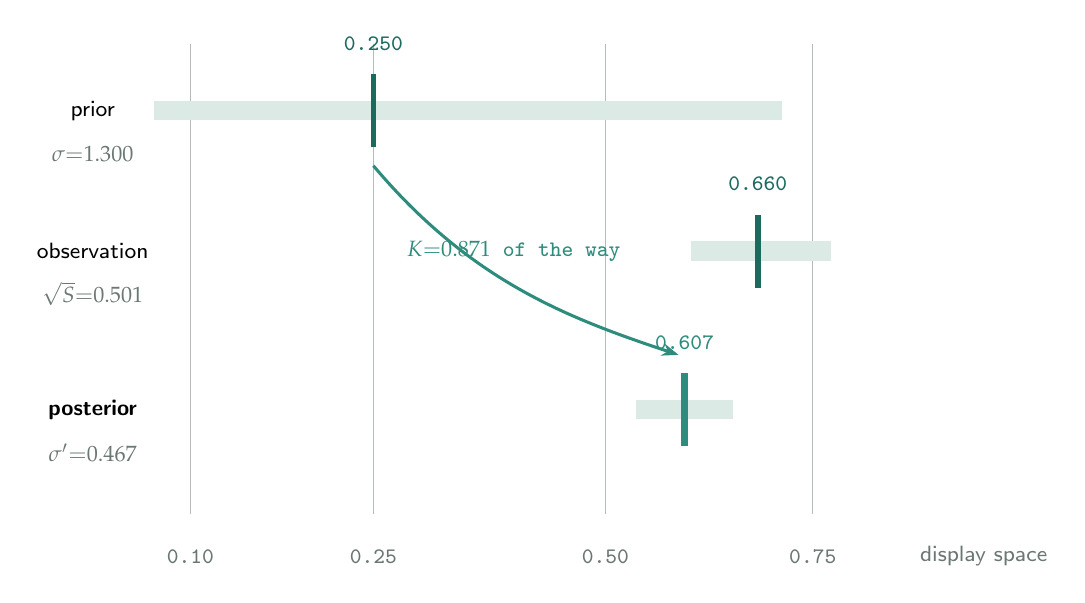
\begin{tikzpicture}[x=1.55cm, y=1.55cm,
    lab/.style={font=\sffamily\footnotesize},
    num/.style={font=\ttfamily\footnotesize}]
  % axis in logit space, mapped for display: 0.10 .. 0.75 as tick labels
  \foreach \x/\t in {0.5/0.10, 2.0/0.25, 3.9/0.50, 5.6/0.75} {
    \draw[mutedgray, opacity=.5] (\x,-0.3) -- (\x,3.55);
    \node[num, mutedgray] at (\x,-0.65) {\t};
  }
  \node[lab, mutedgray] at (7.0,-0.65) {display space};

  % prior bar: wide, centered at mu=-1.0986 (x~=2.0)
  \draw[bandfill, line width=7pt] (0.2,3.0) -- (5.35,3.0);
  \draw[accent, line width=2pt] (2.0,2.7) -- (2.0,3.3);
  \node[num, accent] at (2.0,3.55) {0.250};
  \node[lab] at (-0.3,3.0) {prior};
  \node[num, mutedgray] at (-0.3,2.65) {\footnotesize $\sigma{=}1.300$};

  % observation bar: y=0.66 (x~=5.15), narrower
  \draw[bandfill, line width=7pt] (4.6,1.85) -- (5.75,1.85);
  \draw[accent, line width=2pt] (5.15,1.55) -- (5.15,2.15);
  \node[num, accent] at (5.15,2.4) {0.660};
  \node[lab] at (-0.3,1.85) {observation};
  \node[num, mutedgray] at (-0.3,1.5) {\footnotesize $\sqrt{S}{=}0.501$};

  % posterior bar: mu=0.4357 (x~=4.55), sigma=0.467, narrower still
  \draw[bandfill, line width=7pt] (4.15,0.55) -- (4.95,0.55);
  \draw[accent2, line width=2.6pt] (4.55,0.25) -- (4.55,0.85);
  \node[num, accent2] at (4.55,1.1) {\textbf{0.607}};
  \node[lab] at (-0.3,0.55) {\textbf{posterior}};
  \node[num, mutedgray] at (-0.3,0.2) {\footnotesize $\sigma'{=}0.467$};

  \draw[accent2, -{Stealth[length=6pt]}, line width=1.1pt]
       (2.0,2.55) .. controls (2.8,1.6) and (3.6,1.3) .. (4.5,1.0);
  \node[num, accent2] at (3.15,1.85) {\footnotesize $K{=}0.871$ of the way};
\end{tikzpicture}
\caption{One update, to scale, on a shared logit axis. The prior's interval
is so wide that a single moderately reliable observation pulls the belief
$87\%$ of the way across --- and the posterior comes out narrower than
\emph{either} input, which is what a Bayesian update does. The axis is
uniform in logit space, so the display-space ticks are unevenly spaced.}
\label{fig:kalman}
\end{figure}

% ---------------------------------------------------------------------------
\subsection{S5 --- The Decay Model}
\label{sec:s5}

Time is not evidence, so time must never sharpen a belief. Between
observations the variance grows linearly and the mean reverts toward the
prior, coupled so that one swept constant governs both instead of three
independent knobs.

\begin{keyeq}
\begin{align*}
\sigma^2(t) &= \sigma^2(\tau_{\text{last}}) + \lambda_s\,\Delta t
   & \text{uncertainty grows, always}\\[3pt]
\mu(t) &= \mu + (\mu_0-\mu)\Big(1-e^{-\Delta t\,\lambda_s/k}\Big)
   & \text{mean-reverts toward the prior}\\[3pt]
k &= 0.35, \qquad \tau_s = k/\lambda_s
   & \text{reversion tied to volatility}
\end{align*}
\end{keyeq}

The consequence is worth stating in words, because it is the sentence a
candidate deserves to hear: \textbf{a score falls with time because the
system knows less, not because anyone decided the person got worse.} The
mean drifts back toward ``unknown'' and the interval widens, and both
effects are visible in the \texttt{explain} response as a day count and a
half-life.

\begin{figure}[H]
\centering
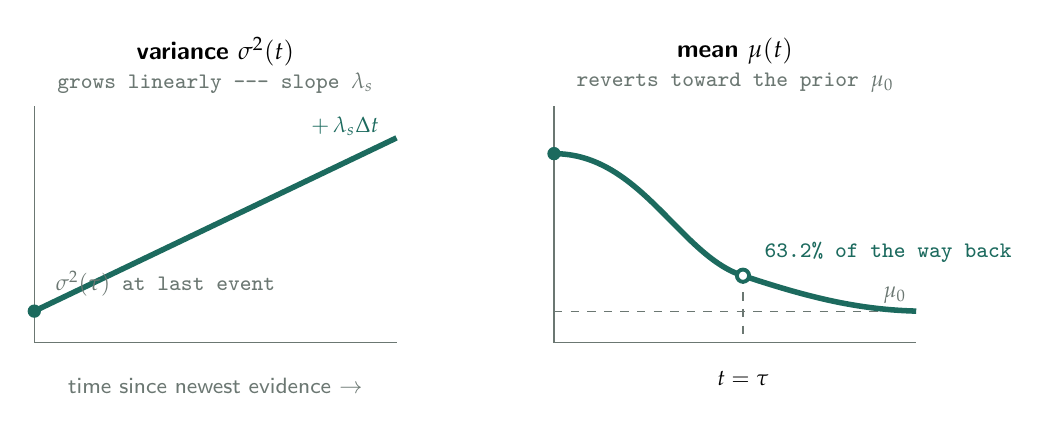
\begin{tikzpicture}[x=1.0cm,y=1.0cm]
  % LEFT panel: variance grows linearly
  \begin{scope}
    \node[font=\sffamily\bfseries\small] at (2.3,3.7) {variance $\sigma^2(t)$};
    \node[font=\ttfamily\footnotesize, mutedgray] at (2.3,3.3) {grows linearly --- slope $\lambda_s$};
    \draw[mutedgray] (0,0) -- (4.6,0);
    \draw[mutedgray] (0,0) -- (0,3.0);
    \draw[accent, line width=2pt] (0,0.4) -- (4.6,2.6);
    \filldraw[accent] (0,0.4) circle (2.2pt);
    \node[font=\ttfamily\footnotesize, mutedgray, anchor=west] at (0.15,0.75)
         {$\sigma^2(\tau)$ at last event};
    \node[font=\ttfamily\footnotesize, accent, anchor=east] at (4.5,2.75)
         {$+\,\lambda_s\Delta t$};
    \node[font=\sffamily\footnotesize, mutedgray] at (2.3,-0.55)
         {time since newest evidence $\to$};
  \end{scope}
  % RIGHT panel: mean reversion
  \begin{scope}[xshift=6.6cm]
    \node[font=\sffamily\bfseries\small] at (2.3,3.7) {mean $\mu(t)$};
    \node[font=\ttfamily\footnotesize, mutedgray] at (2.3,3.3) {reverts toward the prior $\mu_0$};
    \draw[mutedgray] (0,0) -- (4.6,0);
    \draw[mutedgray] (0,0) -- (0,3.0);
    \draw[mutedgray, dashed] (0,0.4) -- (4.6,0.4);
    \node[font=\ttfamily\footnotesize, mutedgray, anchor=east] at (4.6,0.6) {$\mu_0$};
    \draw[accent, line width=2pt]
      (0,2.4) .. controls (1.1,2.4) and (1.6,1.1) .. (2.4,0.85)
              .. controls (3.3,0.55) and (3.9,0.42) .. (4.6,0.4);
    \filldraw[accent] (0,2.4) circle (2.2pt);
    \draw[mutedgray, dashed] (2.4,0.85) -- (2.4,0);
    \filldraw[white,draw=accent, line width=1.4pt] (2.4,0.85) circle (2.2pt);
    \node[font=\ttfamily\footnotesize] at (2.4,-0.45) {$t=\tau$};
    \node[font=\ttfamily\footnotesize, accent, anchor=west] at (2.55,1.15)
         {63.2\% of the way back};
  \end{scope}
\end{tikzpicture}
\caption{Two effects, one constant (schematic). Variance grows without
bound while the mean asymptotes at the prior --- so a very old belief
converges on ``we do not know,'' never on ``this person is bad.'' Because
$\tau=k/\lambda$, choosing a volatility tier sets both rates at once.}
\label{fig:decay}
\end{figure}

% ---------------------------------------------------------------------------
\subsection{S6 --- The Propagation Model}

Evidence for C++ says something about C. Propagation is how that is
expressed, and it is fenced in three ways: it runs at \textbf{read time} so
nothing inferred is ever stored; it goes \textbf{one hop}; and it draws only
from states that have \textbf{direct evidence}. Those three together make
the pass non-iterative and loop-free without needing cycle detection at
all.

\begin{keyeq}
\[
\sigma^2_{\text{pseudo}} = \frac{\sigma^2_{\text{source}}}{\gamma}
\qquad \text{then the ordinary S4 update, unchanged}
\]
\end{keyeq}

Damping reuses the observation mechanism instead of adding a second one.
Weak evidence and distant evidence become the same kind of thing, which is
precisely why they can share an update rule. An inferred skill is presented
with \texttt{evidence\_count: 0}, \texttt{basis: "propagated"}, and the edge
it came along --- never clamped, never disguised as measurement.

\begin{figure}[H]
\centering
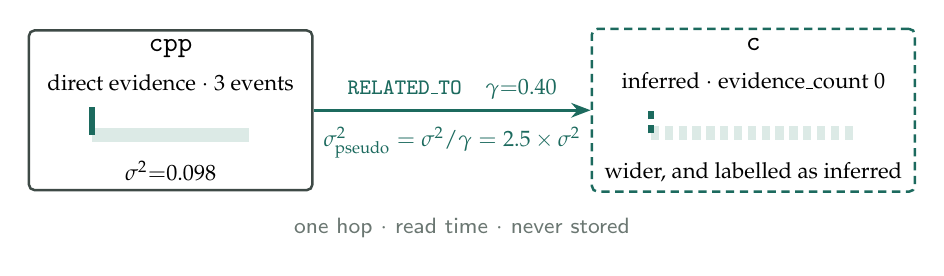
\begin{tikzpicture}[
    box/.style={draw=inkgray, line width=0.9pt, rounded corners=2pt,
                minimum height=1.5cm, minimum width=3.6cm, align=center},
    dashedbox/.style={draw=accent, line width=0.9pt, rounded corners=2pt,
                       dash pattern=on 3pt off 2pt,
                       minimum height=1.5cm, minimum width=4.1cm, align=center},
  ]
  \node[box] (cpp) at (0,0)
    {\ttfamily cpp \\[2pt] \footnotesize direct evidence $\cdot$ 3 events \\[4pt]
     \tikz{\draw[bandfill,line width=5pt](-1.0,0)--(1.0,0); \draw[accent,line width=2pt](-1.0,0)--(-1.0,0.35);}
     \\[2pt] \footnotesize\ttfamily $\sigma^2{=}0.098$};
  \node[dashedbox] (c) at (7.4,0)
    {\ttfamily c \\[2pt] \footnotesize inferred $\cdot$ evidence\_count 0 \\[4pt]
     \tikz{\draw[bandfill,line width=5pt](-1.3,0)--(1.3,0); \draw[accent,line width=2pt](-1.3,0)--(-1.3,0.35);}
     \\[2pt] \footnotesize wider, and labelled as inferred};
  \draw[accent, -{Stealth[length=7pt]}, line width=1.2pt] (cpp.east) -- (c.west)
    node[midway, above, font=\ttfamily\footnotesize, accent] {RELATED\_TO \ $\gamma{=}0.40$}
    node[midway, below=2pt, font=\footnotesize] {$\sigma^2_{\text{pseudo}} = \sigma^2/\gamma = 2.5\times\sigma^2$};
  \node[font=\footnotesize\sffamily, mutedgray] at (3.7,-1.5)
    {one hop $\cdot$ read time $\cdot$ never stored};
\end{tikzpicture}
\caption{Damping is variance inflation. The weakest edge type divides
confidence by the most: $\gamma=0.40$ means the neighbour arrives $2.5\times$
less certain than it actually is. A skill that already has direct evidence
is never overwritten by an inference --- real evidence always wins.}
\label{fig:propagation}
\end{figure}

% ---------------------------------------------------------------------------
\subsection{S7 --- The Display Model: The Published Number is a Lower Bound}

\begin{keyeq}
\[
\text{score} = \sig(\mu - z\sigma), \qquad z = 1.0
\]
\end{keyeq}

What a client sees is not the mean. It is the \textbf{lower end of a
one-sigma interval}, and this single choice does most of the ethical work in
the module. A developer with thin evidence and a developer with abundant
evidence can share a mean; only the second gets a high published score,
because only the second's interval has closed up. Uncertainty costs the
candidate something, which is the only arrangement under which
\emph{gathering more evidence} is the way to raise a number.

$\sig$ is monotone, so a bound in logit space is still a bound after the
transform. The interval always travels beside the score in every response,
so it cannot be mistaken for a point estimate.

% ---------------------------------------------------------------------------
\subsection{S8 --- The Fold: How the Seven Parts Compose}

State is a \emph{derived cache and never a source of truth}. Any score is
recomputed from the append-only log on demand, in a total order.

\begin{keyeq}
\begin{alignat*}{2}
&\text{state} &&\gets \text{prior at the first event's date}\\
&\text{for each event bearing on this skill,}\quad&&\text{ordered by } (\text{occurred\_at}, \text{event\_id}):\\
&\quad\text{state} &&\gets \text{decay}(\text{state} \to \text{event date})\\
&\quad\text{state} &&\gets \text{update}(\text{state}, \text{observed}, \sigma^2_{\text{obs}})\\
&\text{state} &&\gets \text{decay}(\text{state} \to \text{as\_of})
\end{alignat*}
\end{keyeq}

Ordering by $(\text{occurred\_at}, \text{event\_id})$ is a total order, so
two events on the same day still fold deterministically. Recomputing rather
than caching is what makes three otherwise expensive things cheap:
\texttt{as\_of} queries against any past date, ablation (fold again with one
event withheld, to show what it was worth), and the parameter sweep.

% ============================================================================
\section{Models 4 and 5: Ordering and Noticing}
\label{sec:query}
\label{sec:integrity}
% ============================================================================

\subsection*{Model 4 --- The Partial-Order Ranking Model}

Search does not return a ranking, because the evidence does not support
one. Two candidates whose intervals overlap are \emph{not distinguishable},
and printing them in an order would invent a fact. So search returns
\textbf{tiers}: within a tier, the API says plainly that it cannot separate
them.

The caller also chooses the risk posture rather than having one chosen
quietly for them: \texttt{definite=true} requires the whole interval to
clear the bar; \texttt{definite=false} requires only that the interval
reaches it.

\begin{figure}[H]
\centering
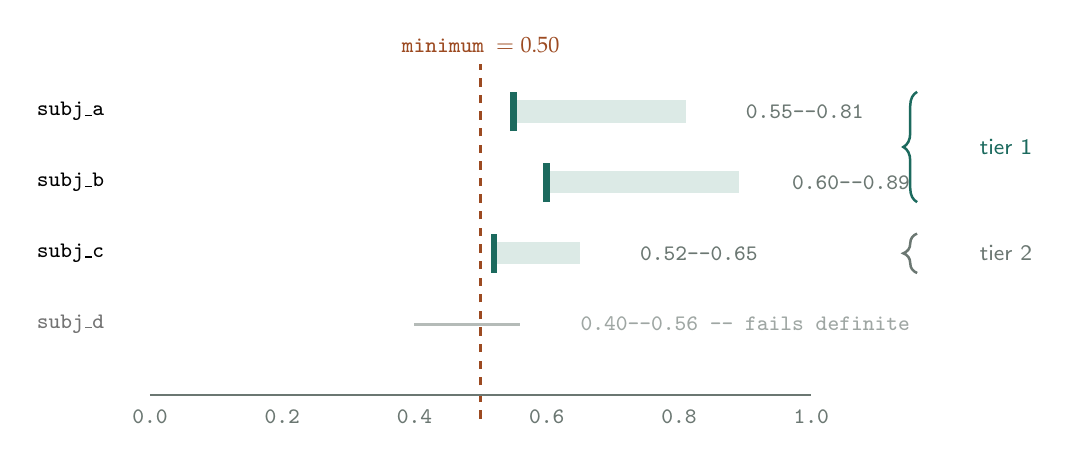
\begin{tikzpicture}[x=8.4cm, y=1.0cm,
    lab/.style={font=\ttfamily\footnotesize},
    num/.style={font=\ttfamily\footnotesize, mutedgray}]
  \draw[negative, dashed, line width=1pt] (0.50,-0.3) -- (0.50,4.2);
  \node[num, negative] at (0.50,4.45) {minimum $=0.50$};

  \node[lab] at (-0.12,3.6) {subj\_a};
  \draw[bandfill, line width=8pt] (0.55,3.6) -- (0.81,3.6);
  \draw[accent, line width=2.4pt] (0.55,3.35) -- (0.55,3.85);
  \node[num] at (0.99,3.6) {0.55--0.81};

  \node[lab] at (-0.12,2.7) {subj\_b};
  \draw[bandfill, line width=8pt] (0.60,2.7) -- (0.89,2.7);
  \draw[accent, line width=2.4pt] (0.60,2.45) -- (0.60,2.95);
  \node[num] at (1.06,2.7) {0.60--0.89};

  \node[lab] at (-0.12,1.8) {subj\_c};
  \draw[bandfill, line width=8pt] (0.52,1.8) -- (0.65,1.8);
  \draw[accent, line width=2.4pt] (0.52,1.55) -- (0.52,2.05);
  \node[num] at (0.83,1.8) {0.52--0.65};

  \node[lab, opacity=.55] at (-0.12,0.9) {subj\_d};
  \draw[mutedgray, opacity=.5, line width=1pt] (0.40,0.9) -- (0.56,0.9);
  \node[num, opacity=.65] at (0.90,0.9) {0.40--0.56 -- fails definite};

  \draw[decorate, decoration={brace, amplitude=5pt, mirror}, accent, line width=0.9pt]
       (1.16,3.85) -- (1.16,2.45);
  \node[font=\sffamily\footnotesize, accent, anchor=west] at (1.24,3.15) {tier 1};

  \draw[decorate, decoration={brace, amplitude=5pt, mirror}, mutedgray, line width=0.9pt]
       (1.16,2.05) -- (1.16,1.55);
  \node[font=\sffamily\footnotesize, mutedgray, anchor=west] at (1.24,1.8) {tier 2};

  \draw[mutedgray] (0,0) -- (1,0);
  \foreach \x/\t in {0/0.0, 0.2/0.2, 0.4/0.4, 0.6/0.6, 0.8/0.8, 1.0/1.0}
    \node[num] at (\x,-0.28) {\t};
\end{tikzpicture}
\caption{A partial order, not a ranking. \texttt{subj\_a} and
\texttt{subj\_b} overlap, so they share a tier and no order is asserted
between them. \texttt{subj\_c} clears the bar in its own tier;
\texttt{subj\_d} reaches the threshold but does not clear it definitely, so
a \texttt{definite} search excludes it. Measurement showed that separating
two candidates whose means differ by $0.10$ needs $z\le 0.40$ --- at the
published $z=1$ this search can filter but honestly cannot rank.}
\label{fig:tiers}
\end{figure}

\subsection*{Model 5 --- The Integrity Model: Nine Rules That Change No Number}

The obvious design is to spot something suspicious and discount the
evidence. That is exactly what this must not do: a signal that silently
moves a score is an unexplainable penalty, and with no overall trust number
there is nowhere for it to hide. So 6.5 produces \textbf{findings}, and a
test asserts the skill graph is byte-identical before and after it runs.

\begin{table}[H]
\centering\small
\begin{tabular}{@{}lcL{6.8cm}@{}}
\toprule
\textbf{Check} & \textbf{Severity} & \textbf{What it notices} \\
\midrule
\texttt{EVIDENCE\_BURST}            & attention & many artefacts appearing in a narrow window \\
\texttt{OWNERSHIP\_UNPROVEN}        & attention & the GitHub identity was never proven \\
\texttt{CONTRADICTED}               & attention & a decisive check failed against a claim \\
\texttt{SINGLE\_SOURCE}             & notice    & a skill resting entirely on one origin \\
\texttt{CLAIM\_ONLY}                & notice    & a skill with nothing but self-report behind it \\
\texttt{INFERRED\_ONLY}             & notice    & a skill reached only by propagation \\
\texttt{WHOLLY\_STALE}              & notice    & all evidence older than the skill's own half-life \\
\texttt{BREADTH\_FROM\_ONE\_ARTEFACT} & notice  & many skills claimed off a single repository \\
\texttt{QUARANTINED\_EVIDENCE}      & notice    & evidence held out because the ontology lacks the node \\
\bottomrule
\end{tabular}
\caption{The nine integrity checks and their severities. There is
deliberately no third, more severe level.}
\end{table}

Three properties are structural. Every finding \textbf{names its
evidence}. Every finding \textbf{carries an innocent explanation} --- a
burst of recent commits is a student finishing coursework far more often
than it is anything else. And there is \textbf{no ``fail'' severity}: two
values only, because a third would invite somebody to threshold on it.

% ============================================================================
\section{End to End: One Real Number, All the Way Through}
\label{sec:worked}
% ============================================================================

Everything above, applied to the skill \texttt{go} for the candidate in the
worked example. Two events, both dated 2026-06-10, queried 81 days later.
These figures are the ones the shipped code emits.

\begin{table}[H]
\centering\footnotesize
\begin{tabular}{@{}L{4.1cm}rrrrrrrr@{}}
\toprule
\textbf{Step} & \textbf{obs.} & $\sigma^2_{\text{obs}}$ & $K$ & $\mu$ & $\sigma$ & \textbf{score} & \textbf{mean} & \textbf{upper} \\
\midrule
prior, no evidence & --- & --- & --- & $-1.0986$ & 1.300 & 0.083 & 0.250 & 0.550 \\
\texttt{repo\_artifact}: distributed-kv, 168 commits, 92\% Go
    & 0.660 & 0.2506 & 0.871 & $+0.4357$ & 0.467 & 0.492 & 0.607 & 0.712 \\
\texttt{claim\_corroborated}: the CV's Go claim, now backed
    & 0.680 & 0.1786 & 0.550 & $+0.6107$ & 0.313 & 0.574 & 0.648 & 0.716 \\
decay to \texttt{as\_of}, $+81$ days
    & --- & --- & --- & $+0.4960$ & 0.350 & \textbf{0.536} & 0.622 & 0.700 \\
projected, if nothing arrives for $+1$ year
    & --- & --- & --- & $+0.1515$ & 0.456 & 0.425 & 0.538 & 0.647 \\
projected, for a full $\tau$ ($1167$ days)
    & --- & --- & --- & $-0.4700$ & 0.670 & 0.242 & 0.385 & 0.550 \\
\bottomrule
\end{tabular}
\caption{The \texttt{go} skill through six fold steps. Reproduced by
\texttt{make demo}; matches \texttt{demo/output/04-explain.json} exactly.}
\label{tab:trace}
\end{table}

\begin{figure}[H]
\centering
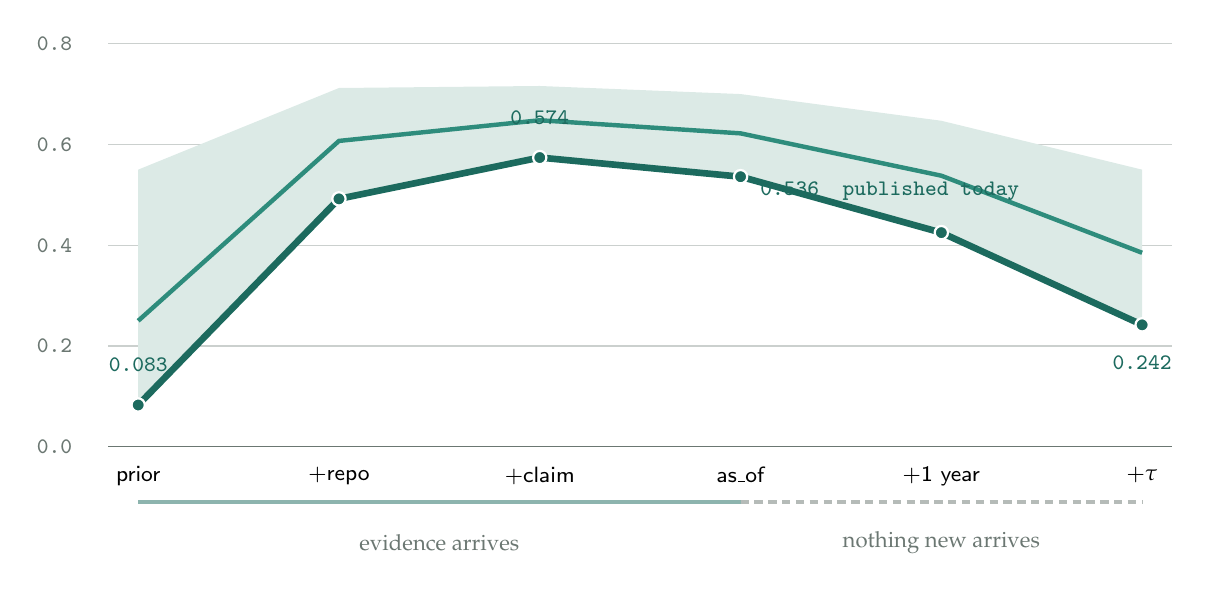
\begin{tikzpicture}[x=2.55cm, y=6.4cm,
    num/.style={font=\ttfamily\footnotesize},
    lab/.style={font=\sffamily\footnotesize}]
  \foreach \y in {0.0,0.2,0.4,0.6,0.8} {
    \draw[mutedgray, opacity=.35] (-0.15,\y) -- (5.15,\y);
    \node[num, mutedgray, anchor=east] at (-0.28,\y) {\y};
  }
  % band polygon: upper edge then lower edge reversed, using upper/score at x=0..5
  \fill[bandfill]
    (0,0.550) -- (1,0.712) -- (2,0.716) -- (3,0.700) -- (4,0.647) -- (5,0.550)
    -- (5,0.242) -- (4,0.425) -- (3,0.536) -- (2,0.574) -- (1,0.492) -- (0,0.083) -- cycle;
  % mean line
  \draw[accent2, line width=1.6pt]
    (0,0.250) -- (1,0.607) -- (2,0.648) -- (3,0.622) -- (4,0.538) -- (5,0.385);
  % score line (emphasized)
  \draw[accent, line width=2.4pt]
    (0,0.083) -- (1,0.492) -- (2,0.574) -- (3,0.536) -- (4,0.425) -- (5,0.242);
  \foreach \x/\y in {0/0.083, 1/0.492, 2/0.574, 3/0.536, 4/0.425, 5/0.242}
    \filldraw[accent, draw=white, line width=0.8pt] (\x,\y) circle (2.4pt);

  \node[num, accent, anchor=south] at (0,0.13) {0.083};
  \node[num, accent, anchor=south, font=\ttfamily\bfseries\footnotesize] at (2,0.62) {0.574};
  \node[num, accent, anchor=north west, font=\ttfamily\bfseries\footnotesize] at (3.05,0.545)
       {0.536 \ published today};
  \node[num, accent, anchor=north] at (5,0.20) {0.242};

  \draw[mutedgray] (-0.15,0) -- (5.15,0);
  \foreach \x/\t in {0/prior, 1/{+repo}, 2/{+claim}, 3/as\_of, 4/{+1 year}, 5/{+$\tau$}}
    \node[lab, anchor=north] at (\x,-0.02) {\t};

  \draw[accent, line width=1.3pt, opacity=.5] (0,-0.11) -- (3,-0.11);
  \draw[mutedgray, densely dashed, line width=1.3pt, opacity=.5] (3,-0.11) -- (5,-0.11);
  \node[lab, mutedgray, font=\footnotesize] at (1.5,-0.19) {evidence arrives};
  \node[lab, mutedgray, font=\footnotesize] at (4,-0.19) {nothing new arrives};
\end{tikzpicture}
\caption{Evidence narrows the band; time widens it. The published score
climbs from $0.083$ to $0.574$ not because the mean moved furthest --- the
mean only reaches $0.648$ --- but because the interval collapsed from
$0.47$ wide to $0.14$. Then it reverses: with nothing new arriving, the band
reopens and the number falls, having never claimed the person got worse.}
\label{fig:trace}
\end{figure}

% ============================================================================
\section{Every Constant, in One Place}
% ============================================================================

Code reads \texttt{value}; the sensitivity sweep reads \texttt{sweep}. Both
come out of the same contract file, so no constant can drift from the one
the sweep tested.

{\small
\begin{longtable}{@{}lL{3.0cm}rrL{4.0cm}@{}}
\toprule
\textbf{Symbol} & \textbf{Name} & \textbf{Value} & \textbf{Sweep range} & \textbf{Governs} \\
\midrule
\endfirsthead
\toprule
\textbf{Symbol} & \textbf{Name} & \textbf{Value} & \textbf{Sweep range} & \textbf{Governs} \\
\midrule
\endhead
$\theta_0$ & prior ability      & 0.25    & 0.15 -- 0.40   & where a developer with no evidence sits \\
$\sigma_0$ & prior sigma        & 1.30    & 0.9 -- 2.0     & how easily the first event moves the belief \\
$S_0$      & observation scale  & 0.10    & 0.05 -- 0.30   & the only free scale in the observation model \\
$z$        & display bound      & 1.0     & 0.5 -- 2.0     & how much uncertainty costs the candidate \\
$k$        & half-life ratio    & 0.35    & 0.15 -- 0.70   & ties mean-reversion to volatility \\
$\lambda$ fundamental & decay rate & $1.0{\times}10^{-4}$ & $3.0{\times}10^{-5}$ -- $3.0{\times}10^{-4}$ & algorithms, C++, data structures \\
$\lambda$ ecosystem   & decay rate & $3.0{\times}10^{-4}$ & $1.0{\times}10^{-4}$ -- $8.0{\times}10^{-4}$ & Python, TypeScript, Go \\
$\lambda$ framework   & decay rate & $7.5{\times}10^{-4}$ & $3.0{\times}10^{-4}$ -- $2.0{\times}10^{-3}$ & React, Docker, PostgreSQL \\
$\gamma$ \texttt{PREREQUISITE\_OF} & damping & 0.55 & 0.3 -- 0.8 & propagation across a prerequisite edge \\
$\gamma$ \texttt{REQUIRES}         & damping & 0.65 & 0.4 -- 0.9 & propagation across a requires edge \\
$\gamma$ \texttt{RELATED\_TO}      & damping & 0.40 & 0.2 -- 0.6 & propagation across a related edge \\
$a,\,b$    & ECDF affine map    & 0.50, 0.40 & --- & rating percentile $\to$ observed ability \\
depth      & propagation hops   & 1       & fixed & never more than one hop, ever \\
\bottomrule
\caption{All fourteen free constants declared in
\texttt{contracts/m6-parameters.yaml}. None is fitted.}
\end{longtable}
}

\begin{notebox}{Known limitation, stated up front}
The Codeforces ECDF is currently \emph{approximated} rather than
regenerated from the real user list --- no network access was available in
the build environment. Every \texttt{platform\_rating} number is therefore
provisional until that table is rebuilt. The contract records this as
\texttt{status: approximated\_pending\_regeneration}, so the caveat travels
with the data rather than living in someone's memory.
\end{notebox}

% ============================================================================
\section{Validation: Checking a Model That Was Never Trained}
% ============================================================================

With no labelled data there is no test-set accuracy to quote, so the model
is checked against a property it must have rather than a benchmark it
should beat: \textbf{if a true ability is known, does the filter recover
it, and is the filter's own stated uncertainty honest?} Three hundred
synthetic developers with known ability, twelve events each, folded through
the shipped code.

\begin{table}[H]
\centering\small
\begin{tabular}{@{}lrl@{}}
\toprule
\textbf{Metric} & \textbf{Measured} & \textbf{Target} \\
\midrule
Bias (mean estimate $-$ mean truth) & $-0.0236$ & $|\text{bias}| < 0.05$ \\
RMSE                                & $0.0510$  & $< 0.15$ \\
Coverage (truth inside $\mu\pm z\sigma$) & $0.677$ & nominal (Gaussian) $= 0.682$ \\
Mean $\sigma$ (logit space)         & $0.2376$  & --- \\
Worst-case $\sigma$                 & $0.1714$  & --- \\
\bottomrule
\end{tabular}
\caption{The recovery gate: \texttt{python3 -m m6\_scoring recover}. \textbf{PASS.}}
\end{table}

The coverage row is the result worth pausing on. A one-sigma interval
around a Gaussian should contain the truth $68.2\%$ of the time. This
filter's intervals contain it $67.7\%$ of the time --- \textbf{the model's
stated uncertainty matches its actual uncertainty}, with nothing tuned to
make that happen. An overconfident filter would score well on RMSE and fail
here, which is exactly why the gate checks coverage and not only error.

\begin{figure}[H]
\centering
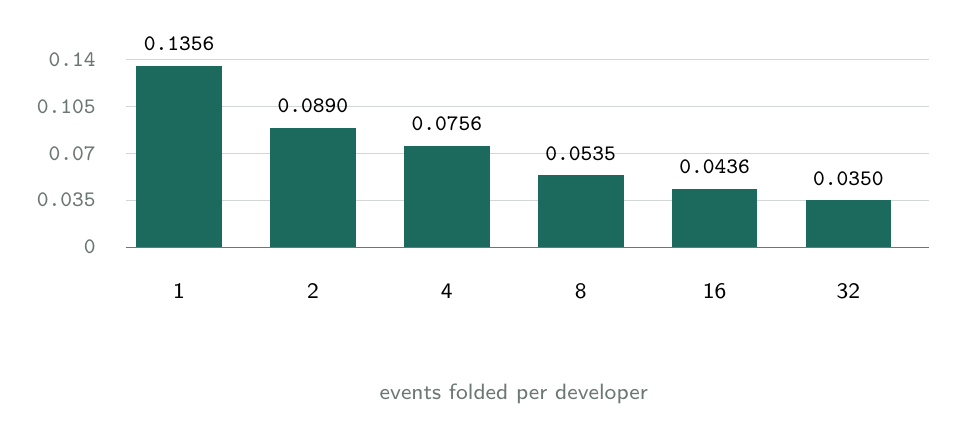
\begin{tikzpicture}[x=1.7cm, y=17cm,
    num/.style={font=\ttfamily\footnotesize},
    lab/.style={font=\sffamily\footnotesize}]
  \foreach \y/\t in {0/0, 0.035/0.035, 0.07/0.07, 0.105/0.105, 0.14/0.14} {
    \draw[mutedgray, opacity=.3] (-0.4,\y) -- (5.6,\y);
    \node[num, mutedgray, anchor=east] at (-0.55,\y) {\t};
  }
  \foreach \i/\v/\t in {0/0.1356/1, 1/0.0890/2, 2/0.0756/4, 3/0.0535/8, 4/0.0436/16, 5/0.0350/32} {
    \fill[accent] (\i-0.32,0) rectangle (\i+0.32,\v);
    \node[num, anchor=south] at (\i,\v+0.004) {\v};
    \node[lab, anchor=north] at (\i,-0.02) {\t};
  }
  \draw[mutedgray] (-0.4,0) -- (5.6,0);
  \node[lab, mutedgray] at (2.5,-0.11) {events folded per developer};
\end{tikzpicture}
\caption{More evidence, less error --- monotonically. Not a benchmark
score: a property the filter has to have. If error ever \emph{rose} with
more evidence, the update rule would be wrong, and no amount of tuning
elsewhere would fix it.}
\label{fig:rmse}
\end{figure}

\subsection*{What the Test Suite Actually Holds}

562 tests, no external test framework required. The interesting ones are
not the assertions that a number equals a number --- they are the ones that
would fail if a stated principle stopped being true: that a suppressed
claim is still reported to the candidate; that the graph is byte-identical
before and after integrity analysis; that one developer's evidence never
folds into another's; that a quarantined skill never reaches a score.

The models themselves were audited by \textbf{mutation testing}: make a
submodule lie, run all 562 tests, and see who notices. That found a real
gap. Making the ontology forget every skill's tier broke only two tests,
one of which was the ontology testing itself --- the scoring engine has a
fallback tier list, so a broken ontology produced \emph{plausible numbers
computed from the wrong half-life}, the worst possible failure shape, with
nothing positioned to doubt them. There is now a test that folds identical
evidence under two ontologies differing only in one skill's tier, and
asserts the score, the variance, and the interval width all move.

% ============================================================================
\section{Known Limitations and Open Work}
% ============================================================================

\pointitem{The ECDF.}{Regenerate the Codeforces reference distribution from
the real user list. Blocks publishing any \texttt{platform\_\allowbreak rating} number
as final.}

\pointitem{The sensitivity sweep.}{Run the full sweep and the ablation
table across all fourteen constants. The machinery exists ---
\texttt{make sweep} enumerates every swept parameter --- but the results
are not yet written up.}

\pointitem{The $\tau$ rename.}{Rename \texttt{half\_life\_days} to reflect
that it is the e-folding time constant, or publish $\tau\ln 2$ under the
current name. Arithmetic unaffected either way.}

% ============================================================================
\section{Conclusion}
% ============================================================================

Module 6 answers one question per skill --- what does the evidence support,
and how sure is that --- and refuses to answer the question nobody can
honestly answer, which is how good is this developer overall. Every number
in it traces to a declared constant, a closed-form update, or a lookup
table a reviewer can read without running any code, and the recovery gate
shows that the filter's stated uncertainty is not merely plausible but
measured to be accurate. That is the whole design: not a model trained to
be right, but a model built so that being wrong would be visible.

\bigskip
\noindent{\small\color{mutedgray}
DevBridge Module 6 --- skill graph layer --- six packages, 562 tests
passing. Every figure in this report was reproduced from the committed code
on \today.}

\end{document}
